\documentclass[11pt,a4paper]{article}

\usepackage{amsmath}
\usepackage{amssymb}
\usepackage{graphicx}
\usepackage{booktabs}
\usepackage[margin=1in]{geometry}
\usepackage[colorlinks=true,linkcolor=black,citecolor=black,urlcolor=blue]{hyperref}

\graphicspath{{../img/}}

% --- shorthand --------------------------------------------------------------
\newcommand{\Ca}{\mathrm{Ca}}
\newcommand{\lgamma}{\ell_\gamma}
\newcommand{\dd}{\mathrm{d}}
\newcommand{\mur}{\mu_r}

\title{The Generalized Lubrication Equation as a subgrid
  contact-line model: theory, numerics, and validation}

\author{Vatsal Sanjay\\[2pt]
  \small CoMPhy Lab, Department of Physics, Durham University\\
  \small \texttt{vatsal.sanjay@comphy-lab.org}}

\date{July 2026}

\begin{document}
\maketitle

\begin{abstract}
\noindent
A moving contact line carries a viscous stress that diverges at the solid,
so the interface shape below the smallest resolved scale of a direct
numerical simulation (DNS) cannot be captured on the DNS mesh. This document
sets out a subgrid treatment of that region built on the Generalized
Lubrication Equation (GLE) of Snoeijer, which stays quantitative for steep
interface slopes where classical lubrication theory fails. We record the
derivation and sign conventions of the arc-length GLE system, the two solvers
that share its right-hand side (adaptive Cash--Karp shooting and a
fixed-mesh collocation branch tracer), the calibration used to reproduce the
dip-coating bifurcation diagram of Snoeijer \& Andreotti, the numerical
verification of every component, and the seam that couples the GLE to a
Basilisk two-phase DNS at the grid scale. The whole solver stack is
header-only C99 with no external dependencies.
\end{abstract}

\section{Introduction}

The hydrodynamic model of a moving contact line predicts a shear stress that
grows like $1/r$ towards the contact line, so the viscous dissipation carries
a non-integrable logarithm and no solution exists within continuum
hydrodynamics alone~\cite{huhscriven1971}. A microscopic mechanism must cut
the singularity off; the simplest and the one used here is a Navier slip
length $\lambda$, below which the no-slip condition is relaxed. The physical
consequence is that the interface bends over a range of scales set by
$\lambda$ at the bottom and by the macroscopic geometry (here the capillary
length $\lgamma = \sqrt{\gamma/\rho g}$) at the top --- six or more decades of
arc length for a millimetric bath and a nanometric slip length.

Resolving all of those decades on a single DNS mesh is infeasible. The
strategy adopted here divides the labour by length scale. A subgrid model
carries the viscous bending of the interface from the slip length up to the
DNS grid size $\Delta$; a Basilisk two-phase DNS carries it from $\Delta$ up
to the macroscopic scale. The two are coupled at $\Delta$: each DNS time step
the subgrid model hands the DNS an \emph{apparent} contact angle at the grid
scale, and takes the DNS interface curvature at that scale as its own outer
boundary condition. The subgrid wedge never has to be resolved on the DNS
mesh.

The subgrid model is the GLE of Snoeijer~\cite{snoeijer2006}, a long-wavelength
theory that --- unlike ordinary lubrication theory --- remains quantitative
when the interface is steep, and reduces to lubrication theory in the
small-slope limit. This document covers, in turn: the derivation and
conventions of the GLE in the arc-length form used in the code
(Section~\ref{sec:theory}); the two numerical solvers and the calibration to
the dip-coating problem (Section~\ref{sec:numerics}); the verification of each
component against independent references (Section~\ref{sec:validation}); and
the GLE\,$\leftrightarrow$\,DNS coupling seam (Section~\ref{sec:coupling}).

\section{Theory}
\label{sec:theory}

\subsection{From the wedge expansion to the generalized lubrication equation}

Classical lubrication theory expands the Stokes equations in the interface
slope and is therefore restricted to $|\nabla h| \ll 1$. Snoeijer's
observation is that at low capillary number the physical requirement is not
that the interface be flat, but that its \emph{curvature} vary slowly: surface
tension is strong enough to keep the shape close to that of a straight wedge,
whatever the opening angle~\cite{snoeijer2006}. One therefore expands the
Stokes flow about the Huh--Scriven similarity solution for a wedge of finite,
slowly varying opening angle $\theta(x)$~\cite{huhscriven1971}, treating the
variation of $\theta$ as the perturbation. The small parameter is
$\varepsilon = \Ca^{1/2}$, with $\Ca = \eta U^{*}/\gamma$, and the expansion is
self-consistent as long as
\begin{equation}
  h \, \partial_x \theta \ll 1,
  \label{eq:validity}
\end{equation}
i.e. the interface angle turns over a length long compared with the local film
thickness. There is no restriction on the size of $\theta$ itself.

The result is the generalized lubrication equation (Snoeijer~\cite{snoeijer2006},
Eq.~14),
\begin{equation}
  \partial_x \kappa
  = 3\,\Ca\,\frac{U/U^{*}}{h^{2}}\,F(\theta)
    + \frac{1}{\gamma}\,\partial_x \Phi\big|_{z=h},
  \qquad
  \kappa = \frac{\partial_{xx} h}{(1 + \partial_x h^{2})^{3/2}},
  \label{eq:gle-cartesian}
\end{equation}
with the full curvature $\kappa$ retained (not its small-slope
approximation), the body-force potential $\Phi$, and the mobility factor
(Snoeijer~\cite{snoeijer2006}, Eq.~15)
\begin{equation}
  F(\theta) = \frac{2}{3}\,
  \frac{\tan\theta \, \sin^{2}\theta}{\theta - \cos\theta\sin\theta}.
  \label{eq:Ftheta}
\end{equation}
As $\theta \to 0$, $F(\theta) \to 1$ and Eq.~\eqref{eq:gle-cartesian} collapses
onto the ordinary lubrication equation, so the GLE is a slope-dependent
correction of the viscous term that is exact at leading order in $\varepsilon$
for any slope.

\subsection{The arc-length system}

Parameterising the interface by its curvature keeps
Eq.~\eqref{eq:gle-cartesian} single-valued through overhangs and folds, which
the Cartesian form cannot represent. Let $s$ be the arc length along the
liquid--gas interface, measured from the contact line, and take the state
vector $y = (h, \theta, \omega, \zeta)$, with $h$ the film thickness normal to
the plate, $\theta$ the local interface inclination, $\omega = \dd\theta/\dd s$
the curvature, and $\zeta$ the distance travelled along the plate. The GLE
becomes the first-order system
\begin{equation}
  \frac{\dd h}{\dd s} = \sin\theta, \qquad
  \frac{\dd\theta}{\dd s} = \omega, \qquad
  \frac{\dd\omega}{\dd s}
    = \frac{3\,\Ca\,M(\theta,\mur)}{h\,(h + 3\lambda)} + G(\theta), \qquad
  \frac{\dd\zeta}{\dd s} = \cos\theta.
  \label{eq:arclength}
\end{equation}
The denominator $h(h+3\lambda)$ is the Navier-slip regularisation of the bare
$h^{2}$: it removes the contact-line singularity of the viscous term while
recovering $h^{2}$ for $h \gg \lambda$. In the one-fluid, small-angle limit the
third equation reduces to $h''' = 3\,\Ca/h^{2}$ with $h^{2}\to h(h+3\lambda)$,
the classical slip-regularised lubrication equation.

\subsection{The two-fluid Huh--Scriven mobility}

For a passive outer fluid the mobility is $F(\theta)$ of
Eq.~\eqref{eq:Ftheta}. The code carries the full two-fluid Huh--Scriven wedge
factor, which accounts for viscous dissipation in the displaced phase at a
gas/liquid viscosity ratio $\mur$~\cite{chan2012}:
\begin{equation}
  M(\theta,\mur) = \frac{2\sin^{3}\theta\,
    \bigl[\mur^{2} f_1(\theta) + 2\mur f_3(\theta) + f_1(\pi-\theta)\bigr]}
   {3\,\bigl[\mur\, f_1(\theta) f_2(\pi-\theta)
     + f_1(\pi-\theta) f_2(\theta)\bigr]},
  \label{eq:mobility}
\end{equation}
with
\begin{equation}
  f_1(\theta) = \theta^{2} - \sin^{2}\theta, \qquad
  f_2(\theta) = \theta - \sin\theta\cos\theta, \qquad
  f_3(\theta) = \theta(\pi-\theta) + \sin^{2}\theta.
  \label{eq:fdefs}
\end{equation}
The \emph{plus} sign in the denominator of Eq.~\eqref{eq:mobility} is
load-bearing: a minus sign there flips the sign of the entire viscous term at
small $\mur$, and every earlier C port in this repository's history carried
that error. In the one-fluid limit ($\mur = 0$) the general form reduces to
\begin{equation}
  M(\theta,0) = \frac{2\sin^{3}\theta}{3\,f_2(\theta)} = \cos\theta\,F(\theta),
\end{equation}
and $M \to 1$ as $\theta \to 0$, recovering the classical result. The mobility
is not named \texttt{f} in the code because in Basilisk \texttt{f} is the
volume-of-fluid volume fraction.

\subsection{Sign conventions and the flat-film consistency check}

We take $\Ca = \eta U/\gamma > 0$ for a \emph{receding} contact line --- the
dip-coating configuration in which the plate is withdrawn from the bath ---
and $\Ca < 0$ for an advancing line. The consistency check is the flat-film
limit of the vertical plate: setting $\theta \to 0$ and $\omega' \to 0$ in
Eq.~\eqref{eq:arclength} balances the viscous term against gravity and gives
the entrained-film thickness
\begin{equation}
  h_{\mathrm{film}} = \sqrt{3\,\Ca}\;\lgamma,
  \label{eq:hfilm}
\end{equation}
the well-known result recovered by Snoeijer~\cite{snoeijer2006} (Fig.~3 of that
paper) for a film dragged down a vertical plate against a receding contact
line.

Gravity enters through
\begin{equation}
  G(\theta) = -\,g^{*}\cos\theta \quad\text{(vertical plate)}, \qquad
  G(\theta) = +\,g^{*}\sin\theta \quad\text{(horizontal plate)},
\end{equation}
with $g^{*} = (\lgamma/\ell_{\mathrm{unit}})^{2}$ the gravity prefactor:
$g^{*} = 1$ when lengths are measured in capillary lengths, and $g^{*} = 0$
disables gravity (the length unit is then free). Retaining $g^{*}$ as a general
scaling rather than fixing it to unity makes the gravity-rescaling invariance
of Section~\ref{sec:validation} an explicit test rather than an identity. In
the vertical geometry $s$ runs from the contact line \emph{down} towards the
bath, so the elevation is $z(s) = \Delta - \zeta(s)$ and the static far field
obeys the hydrostatic balance $\omega = g^{*} z$.

\subsection{The oscillatory film tail and small negative angles}

On the upper (film) branch of the dip-coating problem the interface joins the
meniscus through an oscillatory tail, the classical dimple oscillation of a
Landau--Levich film, in which $\theta$ dips slightly below zero. The mobility
must therefore be continued to small negative angles, and how it is continued
depends on $\mur$. In the one-fluid limit $M(\theta,0) = 2\sin^{3}\theta/
[3 f_2(\theta)]$ is analytically \emph{even} in $\theta$, so the exact even
extension $M(\theta) = M(|\theta|)$ applies, with $M(0) = 1$. For $\mur > 0$
the mobility is \emph{not} even: near $\theta = 0$ it carries a genuine linear
term,
\begin{equation}
  M(\theta,\mur) = 1 + \frac{3\,\mur\,\theta}{2\pi} + \mathcal{O}(\theta^{2}),
  \label{eq:mobility-small}
\end{equation}
so the raw two-fluid formula is evaluated at the \emph{signed} $\theta$ (the
apparent $0/0$ at $\theta = 0$ is removable and set explicitly to $M = 1$).
Because $f_1$ and $f_2$ lose all significant digits to cancellation for small
arguments ($f_1 \sim \theta^{4}/3$, $f_2 \sim 2\theta^{3}/3$), both switch to
their Taylor series below $\theta = 0.02$, which is also more accurate than the
direct trigonometric form there.

\subsection{The dip-coating boundary-value problem}

The steady meniscus at a withdrawn plate is a two-point boundary-value problem
for the system~\eqref{eq:arclength}. At the inner boundary, the contact line,
\begin{equation}
  h(s_0) = h_0, \qquad \theta(s_0) = \theta_e, \qquad
  \omega(s_0) = \omega_0 \;\text{(unknown)},
\end{equation}
with $\theta_e$ the microscopic (equilibrium) contact angle. The integration
starts at a small but finite $s_0 \sim \lambda$ rather than at $s = 0$ because
the curvature diverges logarithmically at the contact line even with slip; the
contribution of the interval $(0, s_0)$ is a bounded logarithm absorbed into
the calibration.

The outer boundary condition is that the trajectory has landed on the static
meniscus manifold by the matching thickness $h = H$. Static solutions
($\Ca = 0$, vertical plate) conserve the first integral
$\tfrac12\omega^{2} + g^{*}\sin\theta$; the branch connected to a flat bath
($\omega \to 0$, $\theta \to \pi/2$) therefore satisfies
\begin{equation}
  \omega\big|_{h=H} = \sqrt{2\,g^{*}\bigl(1 - \sin\theta\big|_{h=H}\bigr)}.
  \label{eq:outer}
\end{equation}
Matching to Eq.~\eqref{eq:outer} at a moderate $H$ (the code uses $H = 5$) is
legitimate because the viscous term in Eq.~\eqref{eq:arclength} has by then
decayed like $3\,\Ca\,M/h$. The meniscus rise follows from the hydrostatic
balance $\omega = g^{*} z$ on the manifold,
\begin{equation}
  \Delta = \zeta\big|_{h=H} + \omega\big|_{h=H}/g^{*},
  \label{eq:Delta}
\end{equation}
and the apparent contact angle from the classical meniscus-rise relation
$\Delta = \sqrt{2(1 - \sin\theta_{\mathrm{app}})/g^{*}}$
(Snoeijer \& Andreotti~\cite{snoeijer2013}, Eq.~4), i.e.
\begin{equation}
  \theta_{\mathrm{app}} = \arcsin\!\left(1 - \tfrac12 g^{*}\Delta^{2}\right).
  \label{eq:thetaapp}
\end{equation}

The branch $\Delta(\Ca)$ turns at a saddle-node fold at $\Ca^{*}$: there the
apparent angle vanishes, $\theta_{\mathrm{app}} \to 0$, and the rise attains
its critical value. Setting $\theta_{\mathrm{app}} = 0$ in
Eq.~\eqref{eq:thetaapp} gives $\Delta = \sqrt{2/g^{*}}$, i.e.
\begin{equation}
  z_c = \sqrt{2}\;\lgamma
\end{equation}
in capillary-length units. Above $\Ca^{*}$ no steady meniscus exists and a
film is entrained: the Landau--Levich transition, at which the upper branch
approaches the entrained-film thickness of Eq.~\eqref{eq:hfilm}. The existence
of this maximum speed, and the avoided-critical-behaviour structure around it,
were established for this system by Eggers~\cite{eggers2004} and by Snoeijer
\emph{et al.}~\cite{snoeijer2006prl}; the experimental branch is that of Delon
\emph{et al.}~\cite{delon2008}.

\section{Numerical implementation}
\label{sec:numerics}

Two complementary solvers share the right-hand side~\eqref{eq:arclength}. Both
are header-only C99 and need only \texttt{libm} --- no GSL, no SUNDIALS ---
so the same headers compile under a host compiler and under Basilisk's
\texttt{qcc}.

\subsection{Adaptive Cash--Karp integration}

The trajectory spans the slip scale $\lambda \sim 10^{-6}\lgamma$ to the
capillary scale in one integration, and near the contact line
$\dd\omega/\dd s \sim 1/s$, which a fixed step cannot follow. The integrator is
an embedded Cash--Karp Runge--Kutta 5(4) pair with proportional step control.
The step error is measured in the mixed norm
\begin{equation}
  E = \left[\frac{1}{4}\sum_{i=1}^{4}
    \left(\frac{\mathrm{err}_i}{\mathrm{atol} + \mathrm{rtol}\,
      \max(|y_i|,|y_i^{5}|)}\right)^{2}\right]^{1/2},
\end{equation}
a step is accepted when $E \le 1$, and the next step is scaled by
$\min(5,\max(0.2,\,0.9\,E^{-1/5}))$; the same comparison rejects a NaN error
norm, which fails every ordinary inequality. Integration terminates on a
\emph{thickness event} $h = H$, localised to a relative tolerance of
$10^{-13}$ on $h$ by bisection on the final step size. This is how the outer
matching point of the boundary-value problem is hit exactly.

\subsection{Single shooting on the contact-line curvature}

The static-manifold condition~\eqref{eq:outer} reduces the boundary-value
problem to a single scalar equation in the unknown $\omega_0$,
\begin{equation}
  \mathcal{R}(\omega_0) \equiv \omega\big|_{h=H}
    - \sqrt{2\,g^{*}\bigl(1 - \sin\theta\big|_{h=H}\bigr)} = 0,
  \label{eq:residual}
\end{equation}
solved by a damped Newton iteration with a central finite-difference
derivative, falling back to geometric bracket expansion and bisection on
stagnation. Trajectories that leave the physical domain before reaching $H$
return signed penalties chosen so that a collapsing interface
($\theta \to 0$, $h \to 0$) reads as $\omega_0$ too small and a fold-over
($\theta \to \pi$) as $\omega_0$ too large; bisection then still brackets.

The conditioning of Eq.~\eqref{eq:residual} sets a floor on the achievable
residual. The flat-bath fixed point of Eq.~\eqref{eq:arclength} has a growing
mode, so a perturbation at the contact line is amplified downstream like
$e^{s}$. The matching therefore cannot be pushed to large $H$ without losing
all precision, and even at $H = 5$ the residual floor with the default
integrator tolerances is $\sim 10^{-8}$; the Newton tolerance is set at
$5\times10^{-8}$ accordingly. (The alternative far-field condition
$\omega(s_{\max}) = 0$, used only for the cross-validation of
Section~\ref{sec:validation}, has $\mathcal{O}(1)$ sensitivity in $\omega$ and
supports a tolerance of $10^{-11}$.) Shooting is the fast single-solve path and
the engine of the DNS coupling; on the lower branch it is reliable up to
roughly $0.6\,\Ca^{*}$, beyond which the residual window in $\omega_0$ narrows
exponentially towards the fold.

\subsection{Collocation branch tracing through the fold}

Shooting cannot trace the full bifurcation diagram. In the $(\omega_0, \Ca)$
plane the branch makes a hairpin at the fold that is narrower than the shooting
map can resolve: the forward flow \emph{compresses} the separation between
neighbouring branches like $e^{-s}$ while amplifying noise like $e^{+s}$. Deep
on the upper branch the trajectory carries a film section of length
$\sim \Delta$ whose exponential dichotomy makes shooting ill-conditioned in
\emph{both} directions. The chart $(\omega_0, \Ca)$ is therefore degenerate at
the fold.

The branch tracer instead discretises the whole problem on a \emph{fixed} mesh
and parameterises solutions by the meniscus rise $\Delta$, which is monotone
along the entire branch. Nodes $s_i = s_0\,(s_{\mathrm{end}}/s_0)^{\tau_i}$ use
a hybrid grading, logarithmic below $s = 0.3$ (to resolve the slip-to-mesoscale
decades near the contact line) and uniform above (to resolve the film and
meniscus foot, whose widths are $\mathcal{O}(\sqrt{\Ca})$); only the uniform
part dilates with the unknown domain length $s_{\mathrm{end}}$. The cell
residuals are the second-order implicit midpoint rule,
\begin{equation}
  y_{i+1} - y_i - (s_{i+1}-s_i)\,
    \mathbf{f}\!\left(\tfrac12(y_i + y_{i+1})\right) = 0,
\end{equation}
closed by the contact-line conditions, the static-manifold
condition~\eqref{eq:outer} at node $N$, the definition $h_N = H$ (which fixes
$s_{\mathrm{end}}$), and the target rise
$\zeta_N + \omega_N/g^{*} = \Delta^{*}$. The unknowns are the $4(N{+}1)$ node
states together with $\Ca$ and $s_{\mathrm{end}}$; the equations are the $4N$
collocation residuals plus six conditions. The system is square.

The Jacobian is block-bidiagonal of bandwidth seven with two dense border
columns ($\partial/\partial\Ca$ and $\partial/\partial s_{\mathrm{end}}$,
formed by finite differences of the full residual) and two border rows (the
$h_N$ and $\Delta$ conditions). It is solved by the bordering algorithm:
banded LU with partial pivoting on the square band part, three back-solves, and
a $2\times2$ reduced system for the two border unknowns. Because $\Delta$ is
monotone along the branch, marching $\Delta^{*}$ with a secant predictor and an
adaptive step (halved on a failed corrector, grown by $1.4\times$ on fast
convergence) walks straight through the fold with no turning-point handling at
all. This is exactly what the mesh re-adaptation of SciPy's
\texttt{solve\_bvp} inside a continuation loop could not do --- the failure
mode of the historical Python continuation (issues~\#14 and~\#16 of the
repository) --- because a mesh that moves between Newton iterations makes the
extended continuation system inconsistent. A fixed mesh keeps it consistent.
The construction is a stabilised multiple-shooting march in the sense of local
parameterisation continuation~\cite{rheinboldt1980}.

\subsection{Parameters and calibration for Fig.~4b}

The dip-coating problem has two microscopic inputs, the equilibrium angle
$\theta_e$ and the slip length $\lambda$. Both are calibrated against the
vector-digitised theory curve of Fig.~4b of Snoeijer \&
Andreotti~\cite{snoeijer2013}, not measured independently:
\begin{itemize}
  \item $\theta_e = 53.46^{\circ}$, fixed by the static foot
    $\Delta(\Ca \to 0) = \sqrt{2(1 - \sin\theta_e)} = 0.627$;
  \item $\lambda/\lgamma = 7.46\times10^{-6}$, fixed by the digitised fold
    $\Ca^{*} = 10.54\times10^{-3}$. The prediction is only logarithmically
    sensitive to $\lambda$, so this value absorbs the $\mathcal{O}(1)$
    microscopic-cutoff choices; it corresponds to about $11$~nm for silicone
    oil at $\lgamma \approx 1.5$~mm.
\end{itemize}
Because $\lambda$ is calibrated \emph{to} $\Ca^{*}$, recovering $\Ca^{*}$ from
the traced branch is circular by construction and is not a test. The genuine
out-of-sample checks are the fold height $\Delta^{*} = 1.440$ (digitised
$1.446$, not fit to) and the full branch shape, including the upper-branch
approach to the Landau--Levich asymptote, which carries no further free
parameters.

\section{Validation}
\label{sec:validation}

Each component is verified against an independent reference; the cross-solver
and cross-language checks establish that both solvers integrate the same
physics, and the mesh-convergence and gravity-invariance checks establish that
the discretisation is correct and unit-consistent.

\paragraph{Mobility.}
The two-fluid mobility~\eqref{eq:mobility} agrees with the Python reference to
machine precision across $\theta \in (0,\pi)$ and $\mur \in [0,1]$. Below
$\theta = 0.02$ the C series form is in fact \emph{more} accurate than the
direct trigonometric formula, which loses precision to the cancellation in
$f_1$ and $f_2$.

\paragraph{Interface profile.}
Against the historical SciPy \texttt{solve\_bvp} reference solving the
identical boundary-value problem, the interface angle $\theta(s)$ agrees to a
relative error below $2.3\times10^{-4}$ throughout the well-conditioned window.
The far field is a genuinely soft condition: the gain
$\dd\theta(10^{6})/\dd\omega_0 \sim 5\times10^{7}$, so the two solutions may
drift apart in $\theta$ at very large $s$ even though the two right-hand sides
agree to machine precision. This is a property of the boundary-value problem,
not of either implementation.

\paragraph{Shooting versus collocation.}
At equal $\Ca$ the two solvers agree to $\sim 2\times10^{-6}$, confirming that
the fixed-mesh march and the adaptive shot converge to the same solution branch.

\paragraph{Mesh convergence of the fold.}
Refining the collocation mesh at $N = 1250$, $2500$, $5000$ cells gives the
fold location
\begin{center}
\begin{tabular}{cc}
  \toprule
  $N$ & $\Ca^{*}$ \\
  \midrule
  1250 & $1.0543847\times10^{-2}$ \\
  2500 & $1.0543572\times10^{-2}$ \\
  5000 & $1.0543504\times10^{-2}$ \\
  \bottomrule
\end{tabular}
\end{center}
The successive differences fall by a factor of about four as the mesh spacing
halves, confirming the second-order convergence of the implicit-midpoint
discretisation.

\paragraph{Linear algebra.}
The bordered banded-LU solve agrees with a dense reference factorisation to
$\sim 10^{-14}$, and the Cash--Karp tableau reproduces its published
coefficients exactly.

\paragraph{Gravity-rescaling invariance.}
Rescaling the gravity prefactor to $g^{*} = 4$ should halve both the slip
length and the meniscus rise (in the new length unit) while leaving $\Ca$
invariant, since $\Ca$ is dimensionless. The traced branch reproduces this to
$4.5\times10^{-6}$, a direct test that the general $g^{*}$ scaling is carried
consistently through both solvers.

\paragraph{Static limit.}
The $\Ca \to 0$ limit reproduces the static meniscus exactly, as it must, since
the outer condition~\eqref{eq:outer} is the static first integral.

\medskip
Figure~\ref{fig:fig4b} shows the traced branch overlaid on the digitised
reference, and Fig.~\ref{fig:cvspy} the C-versus-Python cross-validation.

\begin{figure}[t]
  \centering
  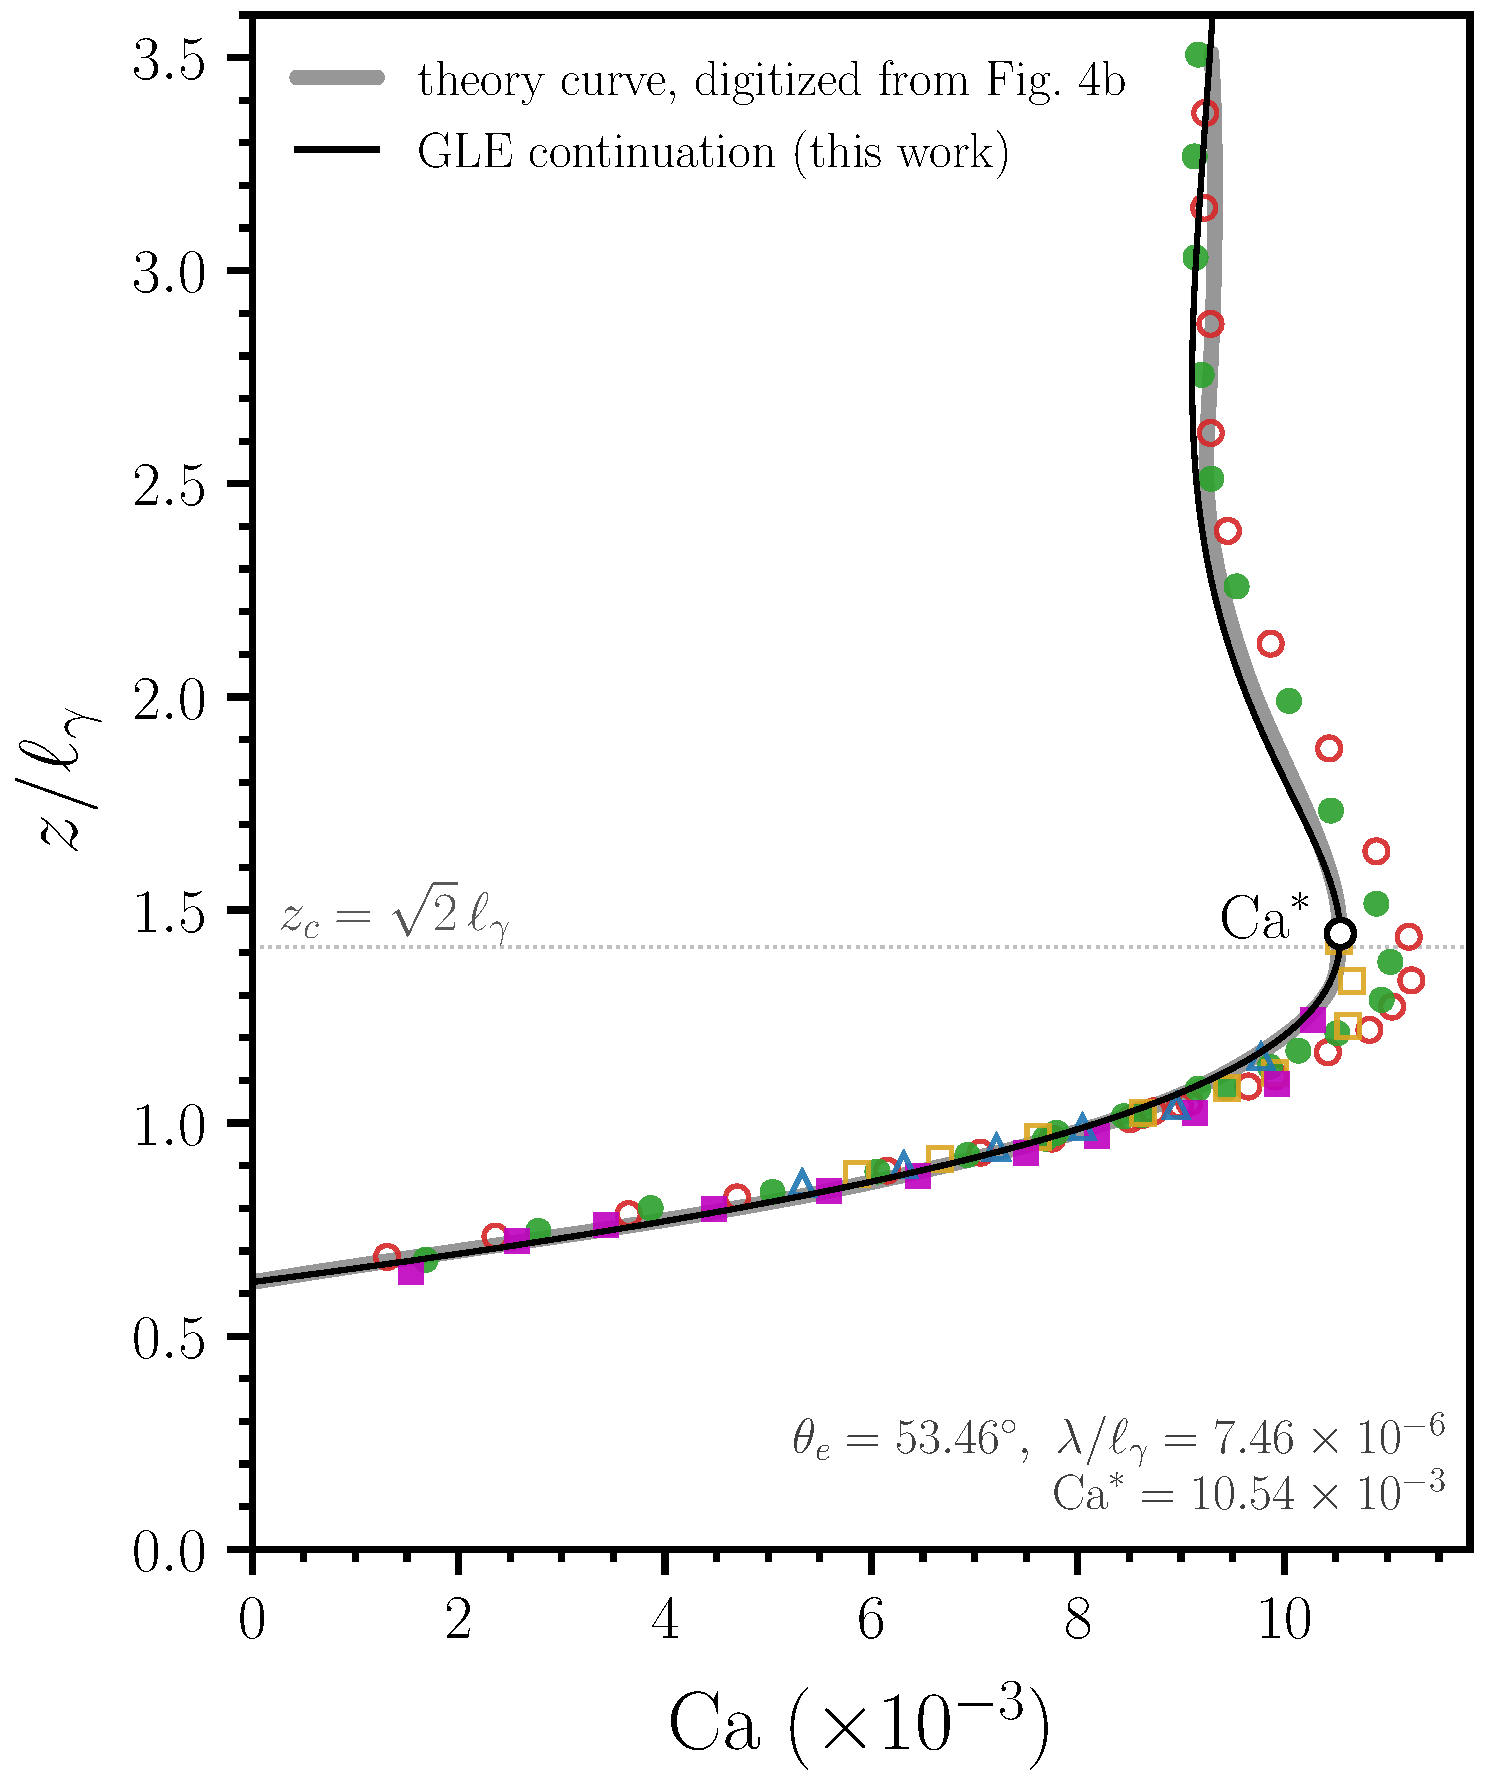
\includegraphics[width=0.72\textwidth]{fig4b-reproduction.pdf}
  \caption{Steady meniscus rise at a receding contact line. Normalised
  contact-line elevation $z/\lgamma$ against capillary number
  $\Ca = \eta U_p/\gamma$ for a partially wetting plate withdrawn from a
  silicone-oil bath. The black line is the present GLE continuation; the thick
  grey line is the multiscale-lubrication prediction digitised from Fig.~4b of
  Snoeijer \& Andreotti (2013)~\cite{snoeijer2013}. Coloured symbols are the
  experimental realizations of Delon et al. (2008)~\cite{delon2008}: each
  colour is a distinct run, and the markers denote steady menisci measured at
  fixed plate speed. In the original review figure these symbols are shadowed
  by thin continuous coloured traces; those are neither theory nor guides to
  the eye, but the continuously recorded transient elevation $z_{cl}(t)$ of
  each run mapped into this plane through the instantaneous relative capillary
  number $\widetilde{\Ca}(t) = \eta(U_p - \dd z_{cl}/\dd t)/\gamma$. Such
  transients relax adiabatically through the succession of quasi-steady states
  and therefore retrace the stationary branch; their visible wiggle is
  measurement noise amplified by the $\dd z_{cl}/\dd t$ term. Only the discrete
  steady-state symbols are digitised here. The branch folds at $\Ca^{*}$: the
  apparent contact angle vanishes, $\theta_{\mathrm{app}} \to 0$, and the rise
  attains $z_c \to \sqrt{2}\,\lgamma$; above $\Ca^{*}$ no steady meniscus
  exists and a film is entrained.}
  \label{fig:fig4b}
\end{figure}

\begin{figure}[t]
  \centering
  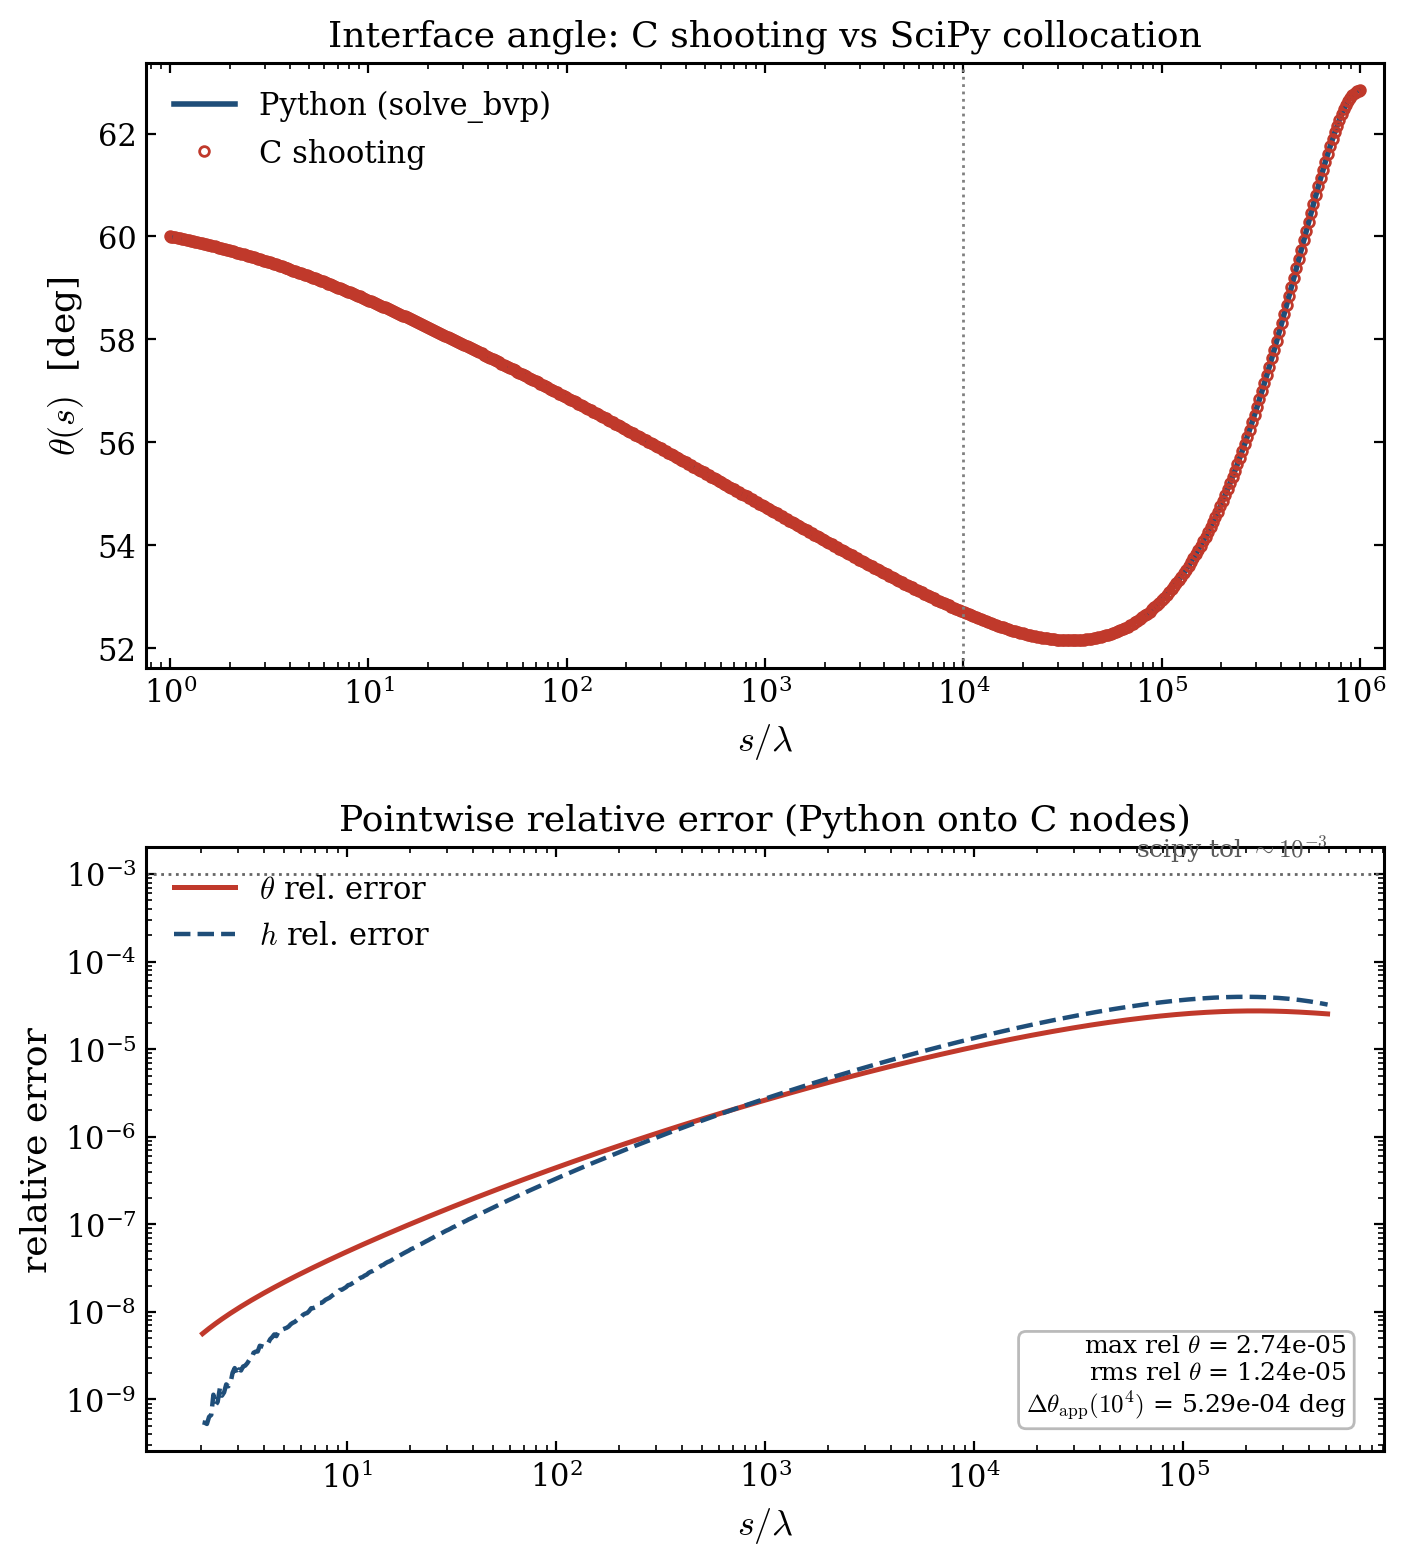
\includegraphics[width=0.95\textwidth]{c-vs-python.png}
  \caption{Cross-validation of the C solver against the historical Python
  \texttt{solve\_bvp} reference on the identical far-field boundary-value
  problem. Left: the interface angle $\theta(s)$ on a logarithmic arc-length
  axis. Right: the relative error between the two solutions on log--log axes.
  Agreement is excellent where the problem is well conditioned
  ($s \lesssim 10^{4}$) and degrades monotonically towards the arc-length cap,
  a consequence of the soft far-field angle condition rather than of either
  implementation.}
  \label{fig:cvspy}
\end{figure}

\section{The DNS and subgrid GLE coupling}
\label{sec:coupling}

The GLE resolves the contact-line region from the slip length up to the DNS
grid size $\Delta$; the Basilisk two-phase DNS resolves everything from
$\Delta$ up to the macroscopic scale. The coupling is a per-time-step event
that exchanges one scalar in each direction at the grid scale. Each step
(\texttt{event (i++)}):
\begin{enumerate}
  \item the DNS interface curvature $\kappa_{\mathrm{DNS}}$ is sampled near the
    contact line at the grid scale;
  \item the subgrid GLE is solved on $s \in [s_0, s_\Delta]$ with
    $h(s_\Delta) = \Delta$, the inner contact-line conditions, and the outer
    condition $\omega(s_\Delta) = \kappa_{\mathrm{DNS}}$, by shooting on
    $\omega_0$;
  \item the resulting apparent angle $\theta_{\mathrm{app}} = \theta(s_\Delta)$
    is imposed on the DNS through the height-function \texttt{contact\_angle()}
    boundary condition.
\end{enumerate}
This is the multiscale strategy of the review~\cite{snoeijer2013} applied as a
grid-scale boundary condition, in the spirit of the mesh-dependent dynamic
contact angle of Afkhami, Zaleski \& Bussmann~\cite{afkhami2009}: the imposed
angle is a property of the resolved scale, not a fixed material constant.

The seam is implemented and runtime-verified. In the demonstration case a
plate is withdrawn at $\Ca = 5\times10^{-3}$ from a bath with microscopic
angle $60^{\circ}$; the imposed angle \texttt{theta\_gle} relaxes to about
$55.9^{\circ}$ in response to the DNS curvature, confirming that the subgrid
solver responds to the resolved interface as intended.

Three problem-specific choices remain before production use, all documented in
the source:
\begin{itemize}
  \item the signed capillary number should be built from the \emph{local}
    contact-line speed (plate speed minus interface speed), not the fixed plate
    speed used in the demonstration;
  \item the sign convention of Basilisk's \texttt{curvature()} must be
    reconciled with the GLE's $\dd\theta/\dd s > 0$ toward-the-bath convention
    before the curvature is handed across;
  \item the coupled system needs a grid-convergence study, the curvature
    sample being currently taken in the interfacial cell nearest the plate.
\end{itemize}
A closed-form flux theory such as that of Luo \& Gao~\cite{luo2025} offers a
further out-of-sample target for the coupled model. The linearised GLE has
separately been checked against the reference data of Kansal \emph{et
al.}~\cite{kansal2024}.

\begin{thebibliography}{99}

\bibitem{huhscriven1971}
C.~Huh and L.~E. Scriven,
\emph{Hydrodynamic model of steady movement of a solid/liquid/fluid contact
line}, J.~Colloid Interface Sci. \textbf{35}, 85--101 (1971).

\bibitem{voinov1976}
O.~V. Voinov,
\emph{Hydrodynamics of wetting},
Fluid Dyn. \textbf{11}, 714--721 (1976).

\bibitem{cox1986}
R.~G. Cox,
\emph{The dynamics of the spreading of liquids on a solid surface. Part 1.
Viscous flow}, J.~Fluid Mech. \textbf{168}, 169--194 (1986).

\bibitem{snoeijer2006}
J.~H. Snoeijer,
\emph{Free-surface flows with large slopes: beyond lubrication theory},
Phys. Fluids \textbf{18}, 021701 (2006).

\bibitem{snoeijer2006prl}
J.~H. Snoeijer, B.~Andreotti, G.~Delon and M.~Fermigier,
\emph{Avoided critical behavior in dynamically forced wetting},
Phys. Rev. Lett. \textbf{96}, 174504 (2006).

\bibitem{delon2008}
G.~Delon, M.~Fermigier, J.~H. Snoeijer and B.~Andreotti,
\emph{Relaxation of a dewetting contact line: experiments and theory},
J.~Fluid Mech. \textbf{604}, 55--75 (2008).

\bibitem{chan2012}
T.~S. Chan, J.~H. Snoeijer and J.~Eggers,
\emph{Theory of the forced wetting transition},
Phys. Fluids \textbf{24}, 072104 (2012).

\bibitem{snoeijer2013}
J.~H. Snoeijer and B.~Andreotti,
\emph{Moving contact lines: scales, regimes, and dynamical transitions},
Annu. Rev. Fluid Mech. \textbf{45}, 269--292 (2013).

\bibitem{eggers2004}
J.~Eggers,
\emph{Hydrodynamic theory of forced dewetting},
Phys. Rev. Lett. \textbf{93}, 094502 (2004).

\bibitem{landau1942}
L.~Landau and B.~Levich,
\emph{Dragging of a liquid by a moving plate},
Acta Physicochim. URSS \textbf{17}, 42--54 (1942).

\bibitem{afkhami2009}
S.~Afkhami, S.~Zaleski and M.~Bussmann,
\emph{A mesh-dependent model for applying dynamic contact angles to VOF
simulations}, J.~Comput. Phys. \textbf{228}, 5370--5389 (2009).

\bibitem{kansal2024}
M.~Kansal \emph{et al.},
\emph{Eur. Phys. J. Spec. Top.} (2024),
\href{https://doi.org/10.1140/epjs/s11734-024-01443-5}
{doi:10.1140/epjs/s11734-024-01443-5}.

\bibitem{luo2025}
K.~Luo and P.~Gao,
\emph{J.~Fluid Mech.} (2025).

\bibitem{rheinboldt1980}
W.~C. Rheinboldt,
\emph{Solution fields of nonlinear equations and continuation methods},
SIAM J.~Numer. Anal. \textbf{17}, 221--237 (1980).

\end{thebibliography}

\end{document}
